%---Include Befehle-------------------------------------------------------------------
\documentclass[a4paper]{article}
\usepackage{ngerman, amsmath, amssymb, bbm, array, tabularx}
\usepackage[T1]{fontenc}
\usepackage[utf8]{inputenc} 		% Kodierung
\usepackage[ngerman]{babel} 		% Sprache
\usepackage{textcomp}       		% Zusätzliche Symbolzeichen 
\setlength{\parskip}{1.5ex plus0.5ex minus0.2ex} 
\setlength{\parindent}{0cm}
\usepackage[]{graphicx}   			% initialisierung von Graphiken
\usepackage{xcolor}					% init von Farbe

%---Seitenränder einstellen-----------------------------------------------------------
\usepackage[left=30mm,right=25mm,top=25mm,bottom=25mm]{geometry}

%---Kopf- und Fusszeile---------------------------------------------------------------
\usepackage{fancyhdr}
\pagestyle{fancy}
\fancyhf{}
\lhead{{\footnotesize HTW Berlin}} 				% linke Seite Kopfzeile, Größe wie eine Fußnote
\chead{} 										% Mitte Kopf - leer
\rhead{{\footnotesize SWE - Belegarbeit GIT}} 	% rechte Seite Kopfzeile
\lfoot{{\footnotesize F. Goerge, S. Ede,\\ R. Peters, J. Meise}} %linke Seite Fußnote
\cfoot{} 										% Mitte Fußnote leer
\rfoot{\thepage} 								% Rechte Fußnote Seitenzahl
\renewcommand{\headrulewidth}{0.2pt}    		% Größe Kopf/Fußzeile?
\renewcommand{\footrulewidth}{0.2pt}

%---Glossar---------------------------------------------------------------------------
\usepackage[urlcolor=blue,colorlinks=true,linkcolor=blue]{hyperref} %Farbe der Links in blau
\usepackage[toc,style=treenoname,order=word,subentrycounter]{glossaries} 
\makeglossaries

%---Glossareinträge-------------------------------------------------------------------
%Glossar update Info. -> Benutzer/in -> Eigene Befehle -> Eigene Befehle editieren
% --> makeindex -s %.ist -t %.glg -o %.gls %.glo
% und unter -> Option -> Texmaker konfigurieren -> Makeindex Verweis aktualisieren!

\newglossaryentry{merge}		{name=Merge		,description={engl. zusammenführen, Vereinigung von Branches}}
\newglossaryentry{Repository}	{name=Repository,description={dt. Lager, Depot, Repositorium. enthält die Geschichte eines Projekts. Jeder Nutzer hat ein eigenes Repository mit der gesamten Geschichte}}
\newglossaryentry{Klone} 		{name=Klone		,description={engl. kopieren}}
\newglossaryentry{Branch}		{name=Branch	,description={engl. Zweig. Ein Entwicklungszweig in der Geschichte}}
\newglossaryentry{Switch}		{name=Switch	,description={engl. wechseln}}
\newglossaryentry{Pull}			{name=Pull		,description={engl. ziehen. Lädt Objekte und Branches. Lädt somit alle Änderungen}}
\newglossaryentry{fetch}		{name=Fetch		,description={engl. holen, holt Brachnes von fernen? Repositories}}
\newglossaryentry{Commit}		{name=Commit	,description={engl. wechseln}}
%-------------------------------------------------------------------------------------

\begin{document}

%---Deckblatt-------------------------------------------------------------------------
\title{\textbf{{\Huge { Belegarbeit GIT \vspace{2cm}} 

\includegraphics[width=\textwidth]{git-logo.png}	% einfügen von Bildern
\vspace{2cm} }}}
\author{Fabian Goerge \\  Sami Ede  \\ Richard Peters \\ Jens Meise}
\date{\today}
\maketitle
\thispagestyle{empty} 								% Keine Seitenzahl auf dem Deckblatt 

%------------------------------------------------------------------------------------

\newpage

%---Inhaltsverzeichnis wird erzeugt--------------------------------------------------
\setcounter{page}{1} 								% Inhaltsverzeichnis startet mit der Seitenzahl 1 
\tableofcontents									% Inhaltsverzeichnis wird erzeugt

%------------------------------------------------------------------------------------

\newpage

\textcolor{red}
{
	FERTIGSTELLUNG BIS 09.12.!!!!!!!!!!! 
	und wehe nicht!!!!!!!!!!!!!\\
	- PDF vollenden (gemeinsame Punkte bearbeiten)\\
	- Präsentation fertigstellen (16.12. / 22.12.)
}
%---Erster Punkt--------------------------------------------------------------------
\section{\underline{Einführung und Ziel der Arbeit}} 	% Section erstellt automatisch den jeweiligen Punkt. Das erste Section erstellt Punkt 1, das 2te Punkt 1 etc.

\subsection{Einführung} 								% Subsection erstellt automatisch Unterpunkte

%Beispiel für einen Glossar Eintrag....der oben noch definiert werden muss!
...mit einem \gls{merge} kann man .....    				% gls = glossary entry; in den Klammern der vordefinierte Glossareintrag

	\textbf{Sami ab hier gehts los...} 					% textbigfat
Was ist Git? Git ist ein Versionsverwaltungssystem. 	
Der Gedanke von Git ist das sich Daten im Laufe der Zeit ändern und Git bietet die Möglichkeit
diese Änderungen zu Verwalten und festzuhalten. (Wer hat wann was und warum geändert?)

\subsection{Ziel}
	Sami...
	Git modellieren, mit den Modellierungsarten auseinandersetzen	
\newpage												% Seitenumbruch
\section{\underline{Textuelle Beschreibung}}

Git ist eine freie Software zur verteilten Versionsverwaltung von Dateien. Git hilft, wenn mehrere Programmierer an einem Projekt arbeiten, indem es verschiedene Features vereint:

  \begin{itemize} 										% Aufzählungen
     
\item Git ermöglicht eine nicht-lineare Entwicklung; das heißt, es ist möglich, an verschiedenen „Positionen“ des Quelltextes zu arbeiten, und diese im Nachhinein automatisch zu vereinen („mergen“). %Jeder Backslash ist ein Bulletpoint
\item des Weiteren bietet Git die Möglichkeit eines lokalen Arbeitens. Jeder User besitzt eine lokale Kopie des kompletten Repositories (inklusive der Versionsgeschichte), so dass auch ohne Anbindung in ein Netzwerk gearbeitet werden kann. Dies ermöglicht sehr schnelles Arbeiten!
Dies bedeutet auch gleichzeitig Multi-Backups! Jeder User speichert die komplette Versionsgeschichte!
\item Mehrere Möglichkeiten, Repositories abzugleichen; Git besitzt ein eigenes Protokoll, und unterstützt unteranderem http, https, ftp und rsync Übertragungen.
\item Versionsgeschichte wird kryptografisch gesichert, so dass es nicht möglich ist, Änderungen an der Versionsgeschichte vorzunehmen, ohne dass sich der Name der Revision ändert.

    \end{itemize} 										% Aufzählung beendet

Des Weiteren bietet Git ein Webinterface.

\section{\underline{Modellierung}}

\subsection{Use-Case-Modell}

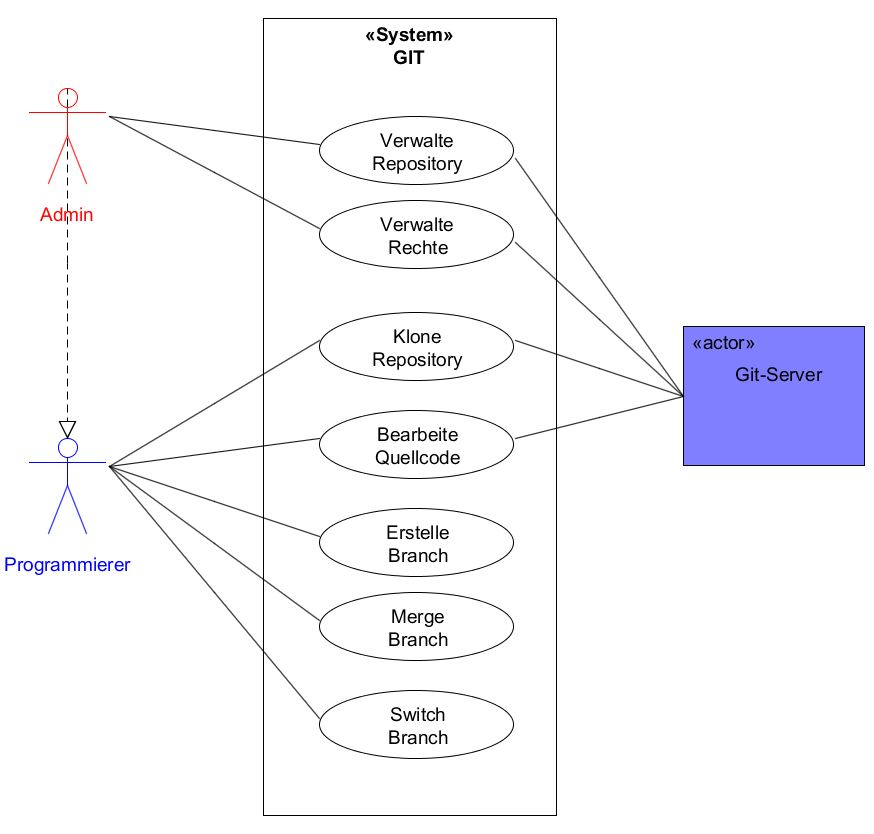
\includegraphics[width=\textwidth]{Use-Case-Modell.png}	

Dieses Use-Cases repräsentieren die Interaktion zwischen dem Programmierer (\textit{Aktor}) und dem Git-System (\textit{Subjekt})\\  							% Textit = Textitalian = kursiv
\\ 														% Absatz
Der Programmierer benutzt das Git-System um ein bestimmtes Ziel zu erreichen. 
Der Git-Server (\textit{Sekundäre Aktor}) wird von dem Git-System genutzt um eine Auswahl von Befehlen ausführen zu können.\\
\\
Der Programmierer repräsentiert eine Personengruppe. An einem Projekt können beliebig viele Programmierer beteiligt seien.  
Der Admin erbt alle Fähigkeiten von dem Programmierer. Demnach kann der Admin auch alle anderen Interaktionen ausüben.  \\
\\
Im Use-Case sind die Möglichkeiten, Verwalte \gls{Repository}, Verwalte Rechte, \gls{Klone} Reopisitory, Bearbeite Quellecode, Erstelle \gls{Branch}, \gls{merge} Branch und \gls{Switch} Branch aufgeführt. \\
\\
Eine detaillierte Beschreibung der Abläufe folgt in den Use-Case-Szenarien. 

\newpage	
\subsubsection{Use-Case-Szenarien (Storys)}

	- Happy day Szenarien und Optionale Verzweigungen (Abweichungen vom Happy Day) (Richard)
	
\textbf{GIT   Use – Case Szenarien}

\textbf{Use Case: 			Clone Repository}\\
Kurzbeschreibung: 	Der Programmierer kopiert sämtliche Daten des Repositories auf seinen lokalen Rechner.\\
Vorbedingung:	Ein Repository muss auf dem Server existieren\\
Primärer Aktor:	Programmierer\\
Nachbedingung:	Das Repository auf dem Rechner des Programmierers ist mit dem auf dem Server identisch\\
Erfolgsszenario:\\
\\
Der Programmierer gibt das Kommando zum Klonen eines Repositories mit Serveradresse in die Shell ein. Das System verbindet sich mit dem Server. Das System überträgt das Repository vom Server auf den Rechner des Programmierers. Das System informiert den Programmierer über den Erfolg der Aktion. Das Use Case endet erfolgreich.\\
\\

\textbf{Use Case: 			Quellcode bearbeiten}\\
Kurzbeschreibung: 	Der Programmierer möchte den Quellcode ändern. Dazu muss er das Repositorie auf den neuesten Stand bringen (‚pull‘), den Quellcode bearbeiten, die Änderungen übernehmen (‚commit‘) und die Änderungen an den Server übertragen (‚Push‘)\\
Vorbedingung:	Ein Repository muss sich auf dem Rechner und auf dem Server befinden.\\
Primärer Aktor:	Programmierer\\
Nachbedingung:	Die Änderungen des Programmierers werden registriert und in die History aufgenommen.\\
Erfolgsszenario:\\
\\
Der Programmierer gibt das Kommando zum Holen von Änderungen in die Shell ein. Das System verbindet sich mit dem Server. Das System vergleicht den lokalen Zustand des Branches mit dem auf dem Server.
Das System integriert (‚\gls{merge}‘) den Branch auf dem Server in den Branch auf dem Rechner. Das System informiert den Programmierer über den Erfolg der Aktion. Der Programmierer ändert den Quellcode
Das System verfolgt die Änderungen. Der Programmierer gibt das Kommando zum Übernehmen (‚Commit‘) von Änderungen in die Shell ein mit einer Kurzbeschreibung seiner Änderungen. Das System übernimmt die Änderungen und trägt sie in die History des aktuellen Branches ein. Das System informiert den Programmierer über den Erfolg der Aktion. Der Programmierer gibt das Kommando zum Übertragen der Änderungen (‚Pull‘) auf den Server ein. Das System integriert den aktuellen Branch des Rechners in den entsprechenden Branch auf dem Server (‚\gls{merge}‘) Das System liefert dem Programmierer eine Erfolgsmeldung. Das Use Case endet erfolgreich.\\
\\
\textbf{Use Case: 			Branch erstellen}\\
Kurzbeschreibung: 	Das System erstellt einen neuen Branch mit dem Zustand des Branches auf dem sich der Programmierer befindet.\\
Vorbedingung:	Es muss ein Repository existieren.\\
Primärer Aktor:	Programmierer\\
Nachbedingung:	Es gibt einen neuen Branch.\\
Erfolgsszenario:\\
\\
Der Programmierer gibt das Kommando zum Erstellen eines Branches in die Shell ein mit dem Namen des neuen Branches. Das System erzeugt einen neuen Branch. Das Use Case endet erfolgreich.\\
\\
\textbf{Use Case: 			Branch mergen}\\
Kurzbeschreibung: 	Ein Branch wird in einen anderen Branch integriert\\
Vorbedingung:	Es müssen 2 Branches existieren.\\
Primärer Aktor:	Programmierer\\
Nachbedingung:	Es gibt einen neuen Branch.\\
Erfolgsszenario:\\
\\
Der Programmierer gibt das Kommando zum Mergen eines Branches in die Shell ein mit dem Namen des zu integrierenden Branches. Das System integriert den Branche in den aktiven Branche. Das Use Case endet erfolgreich.\\
\\
\textbf{Use Case: 			Branch switchen}\\
Kurzbeschreibung: 	Der aktuelle Branch auf dem Rechner wird gewechselt (‚switch‘)\\
Vorbedingung:	Es müssen mindestens 2 Branches existieren.\\
Primärer Aktor:	Programmierer\\
Nachbedingung:	Der aktuelle Branch wurde gewechselt.\\
Erfolgsszenario:\\
\\
Der Programmierer gibt das Kommando zum Wechseln eines Branches (‚switch‘) in die Shell ein mit dem Namen des Zielbranches. Das System wechselt zum Zielbranch.Das Use Case endet erfolgreich.\\
\\
\textbf{Use Case: 			Repository verwalten}\\
Kurzbeschreibung: 	Ein Repository wird verwaltet.\\
Vorbedingung:	Keine – es kann auch erst bei der Verwaltung ein Repository angelegt werden.\\
Primärer Aktor:	Admin\\
Nachbedingung:	Repository verändert. \\
Erfolgsszenario:\\
\\
Der Admin spezifiziert eine Verwaltungsoperation (löschen, erstellen umbenennen). Das System führt die entsprechende Aktion aus und informiert den Admin über den Erfolg der Aktion. Das Use Case endet erfolgreich.\\
\\
\textbf{Use Case: 			Rechte verwalten}\\
Kurzbeschreibung: 	Der Admin kann Leserechte und ausführrecht für bestimmte Nutzergruppen verteilen.\\
Vorbedingung:	Es muss mindestens eine Gruppe bestehen. \\
Primärer Aktor:	Admin\\
Nachbedingung:	Die Rechte wurden geändert. \\
Erfolgsszenario:\\
\\
Der Admin gibt das Kommando zum Verwalten von Rechten in die Shell ein mit dem Namen der zu verwaltenden Gruppe. Das System listet die Rechte der ausgewählten Gruppe. Der Admin gibt entsprechende Kommandos zum Verwalten der Rechte ein. Das System informiert den Admin über eine erfolgreiche Ausführung der Aktion. Das Use Case endet erfolgreich.\\
\\

Repository: Die Projektdaten und Informationen des Git-Systems (History, Branches, etc).
\newpage	
\subsection{Domänenmodell}

	  - Klassendiagramme, Objekte, Verknüpfungen, Abhängigkeiten (Jens, Richard)
\newpage		
\subsection{Ausgewählte Zustandsdiagramme}

	 - Verschiedene Prozesse beschreiben (Quelltext bearbeiten, Branches mergen) (Sami, Fabian)
	 Ick hab jetzt mal für uns einen Branch gemacht... und mir ist gerade nix eingefallen zum ändern.
	 Also nur die Zeile hier.
\newpage	

%---Glossar als subsection und "Glossar" einfügen------------------------------------------
\setglossarysection{subsection}
\printglossary[title={Glossar}, numberedsection]

%------------------------------------------------------------------------------------------
	 - Fachwörter werden erklärt (Repository, Branch, bla...) (Gemeinsam im Laufe der Latexerstellung) 
\newpage		
\section{\underline{Erfahrung aus der Teamarbeit}}

	gemeinsam gewählter Prozess...
	(Gemeinsam)

\section{\underline{Schlussbetrachtung}}
	
	Zusammenfassend kann man sagen das hier noch nicht so viel passiert ist ;)	
	(Gemeinsam)
	.ignore test!
	
\end{document}

